\documentclass[14pt]{article}

\usepackage[utf8]{inputenc}
\usepackage[T1]{fontenc}
\usepackage[english,ngerman]{babel}
\usepackage{graphicx}
\usepackage{amsmath}
\usepackage{amsfonts}
\usepackage{amssymb}
\usepackage{amsthm}

\usepackage{fancyhdr}
\usepackage{lastpage}
\usepackage[left=2.5cm,right=2.5cm,top=1.5cm,bottom=2cm,includeheadfoot]{geometry}
\usepackage[makeroom]{cancel}
\usepackage{titlesec}
\usepackage{enumerate}
\usepackage{url}

\usepackage{extarrows}
\usepackage{float}
\usepackage[table]{xcolor}
\usepackage{listings}
\usepackage[breakable, theorems, skins]{tcolorbox}

\DeclareRobustCommand{\task}[2][gray!20]{
\begin{tcolorbox}[
        breakable,
        left=0pt,
        right=0pt,
        top=0pt,
        bottom=0pt,
        colback=#1,
        colframe=#1,
        width=\dimexpr\textwidth\relax,
        enlarge left by=0mm,
        boxsep=5pt,
        arc=0pt,outer arc=0pt,
        ]
        #2
\end{tcolorbox}
}
\DeclareRobustCommand{\enum}{
\begin{enumerate}[label={\alph*)}]
}
\DeclareRobustCommand{\enumend}{
\end{enumerate}
}


\pagestyle{fancy}
\fancyhead[L]{Machine Learning: Algorithms and Theory \\ SS 18}
\fancyhead[C]{Assignment 10}
\fancyhead[R]{David Barrera \\ Nahoko Kaji}
\fancyfoot[L]{}
\fancyfoot[R]{}
\renewcommand{\headrulewidth}{0.4pt}
\renewcommand{\footrulewidth}{0.4pt}
%\setlength{\headheight}{25.0pt}
\parindent0pt

\begin{document}
\section*{Exercise 2: Implementing k-means and spectral clustering}
(implementation exercise)

\section*{Exercise 3: Design your own exam questions}
\begin{enumerate}

\item Please explain the difference of kernel-PCA(Principal Component Analysis) and PCA. What is the advantage to use kernel?

\item Please judge True or False for following each sentences. \\
$[\qquad]$Principal component analysis does not change the value of the main component depending on whether or not to standardize the data. \\
$[\qquad]$The principal component vector is the eigenvector of magnitude 1 of the correlation matrix \\
$[\qquad]$Principal component analysis is a statistical process that compresses multidimensional information into low dimensional information

\item Please divide into two cluster by k-means.
\begin{table}[h]
	\begin{tabular}{|c|c|c|}
	\hline
	Name & maximal blood pressure & cigarette/Day \\ \hline
	A & 80 & 5 \\ \hline
	B & 60 & 3 \\ \hline
	C & 160 & 8 \\ \hline
	D & 140 & 6 \\ \hline
	E & 100 & 6 \\ \hline
	F & 200 & 10 \\ \hline
	\end{tabular}
\end{table}

\end{enumerate}

\section*{Exercise 1: Spectral graph theory}
Because the Latex Layout function does not correct work,
I show the allocation as following.  \\
a) Picture 1 - 4 \\
b) Picture 5 - 10 \\
c) Picture 11 - 14 \\
d) Picture 15 - 17 \\

\begin{description}
% a
\item[(a)]
\begin{figure}[h]
  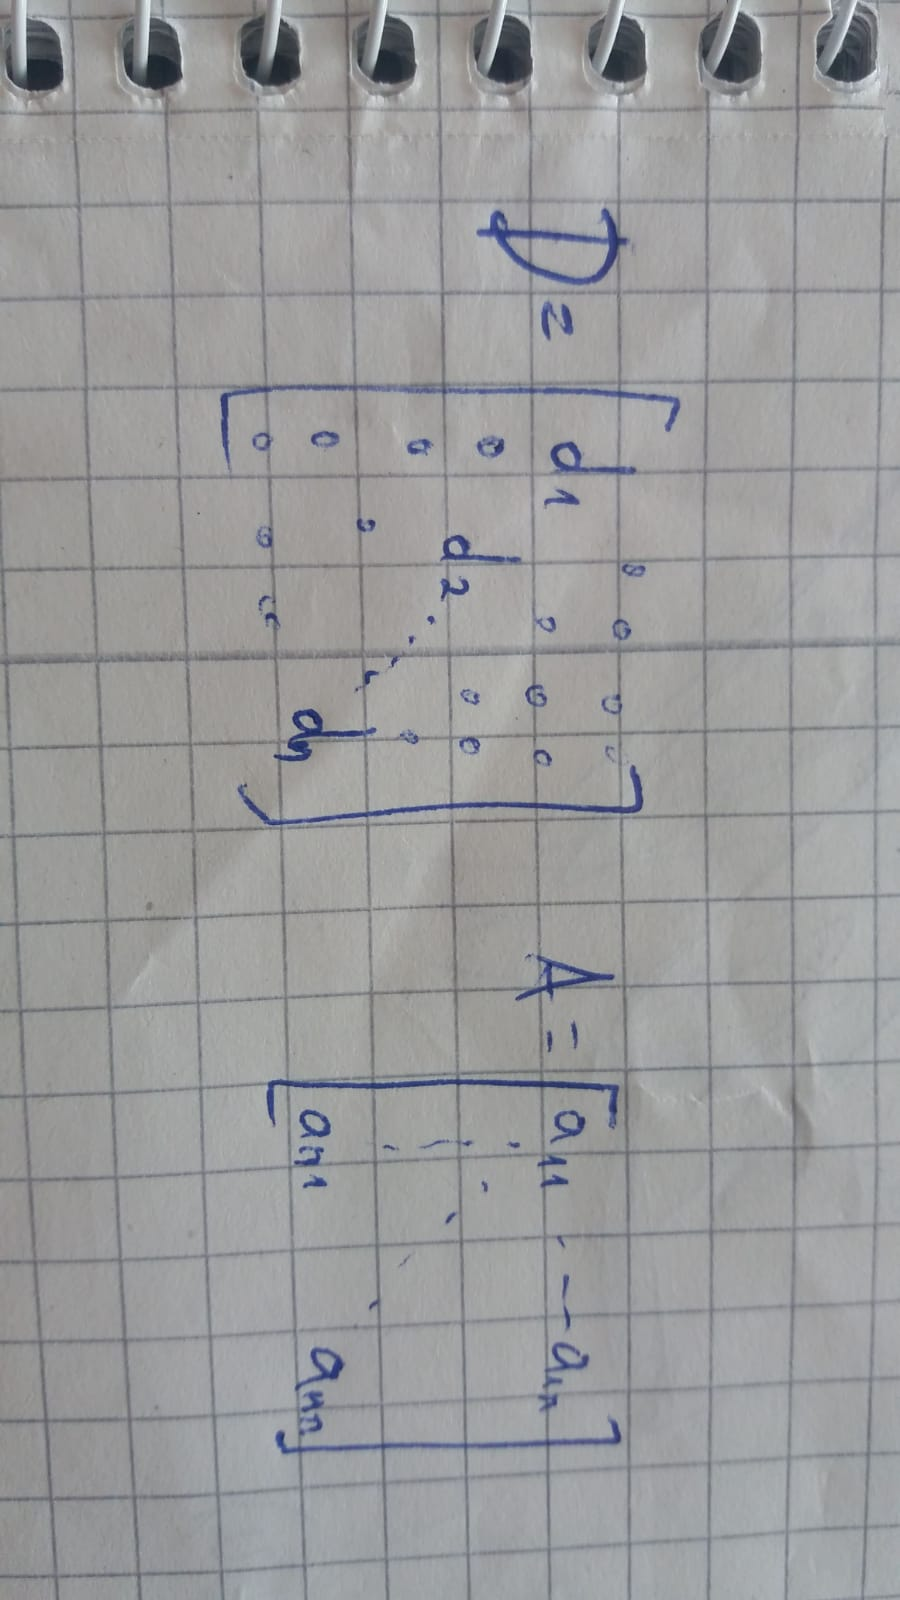
\includegraphics[scale=0.35, angle=90]{a10-ex1-a1.jpeg}
\end{figure}
\begin{figure}[h]
  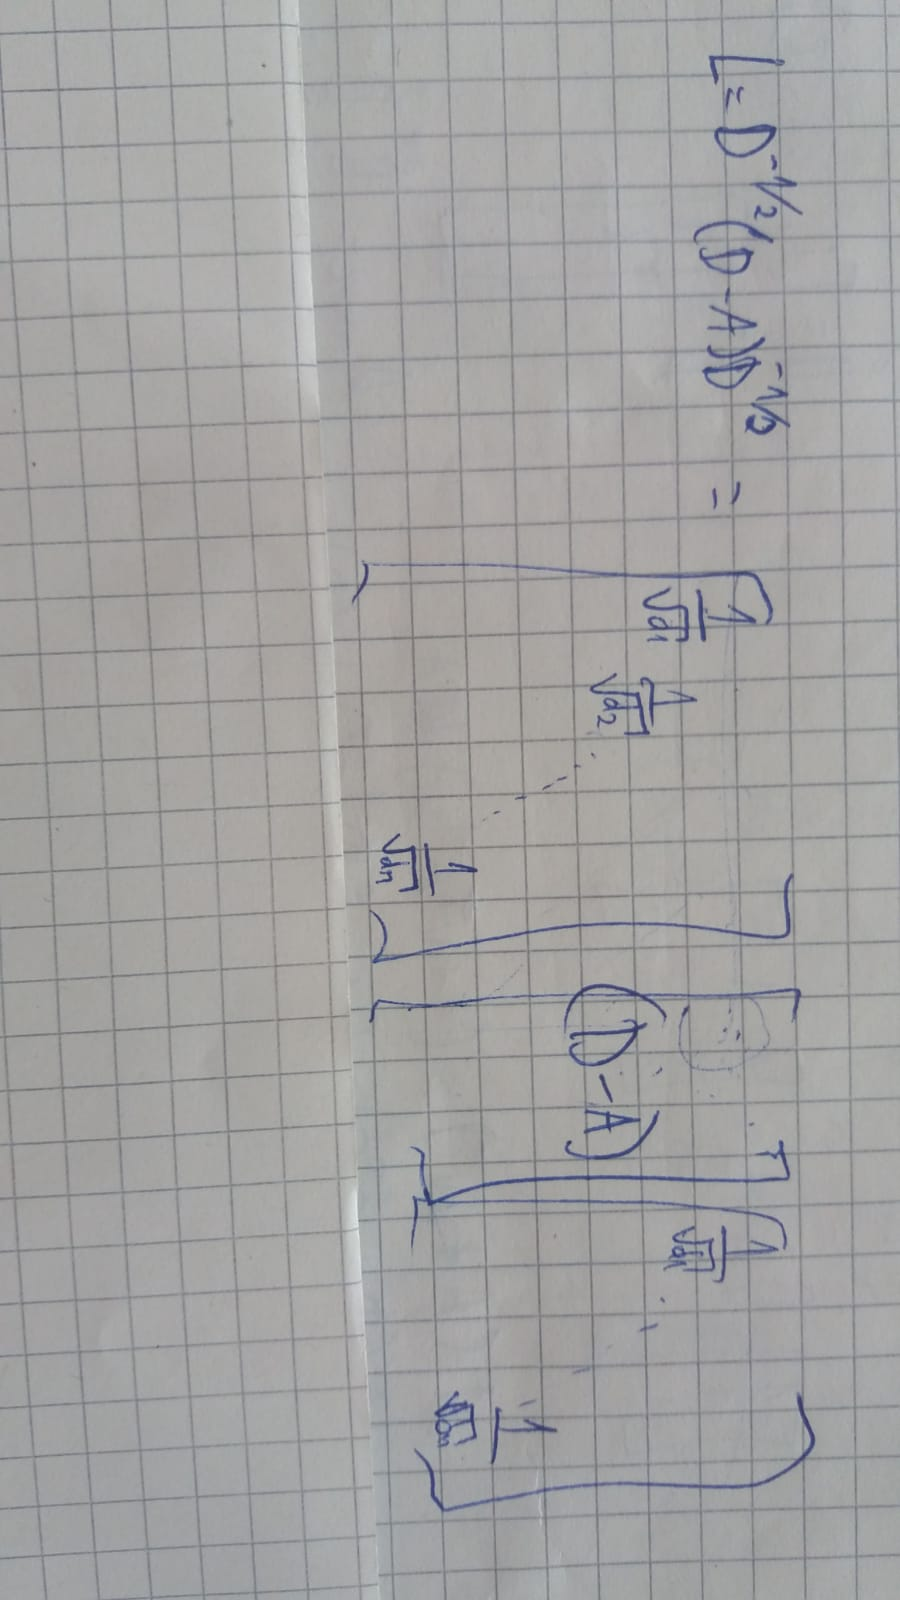
\includegraphics[scale=0.35, angle=90]{a10-ex1-a2.jpeg}
\end{figure}
\begin{figure}[h]
  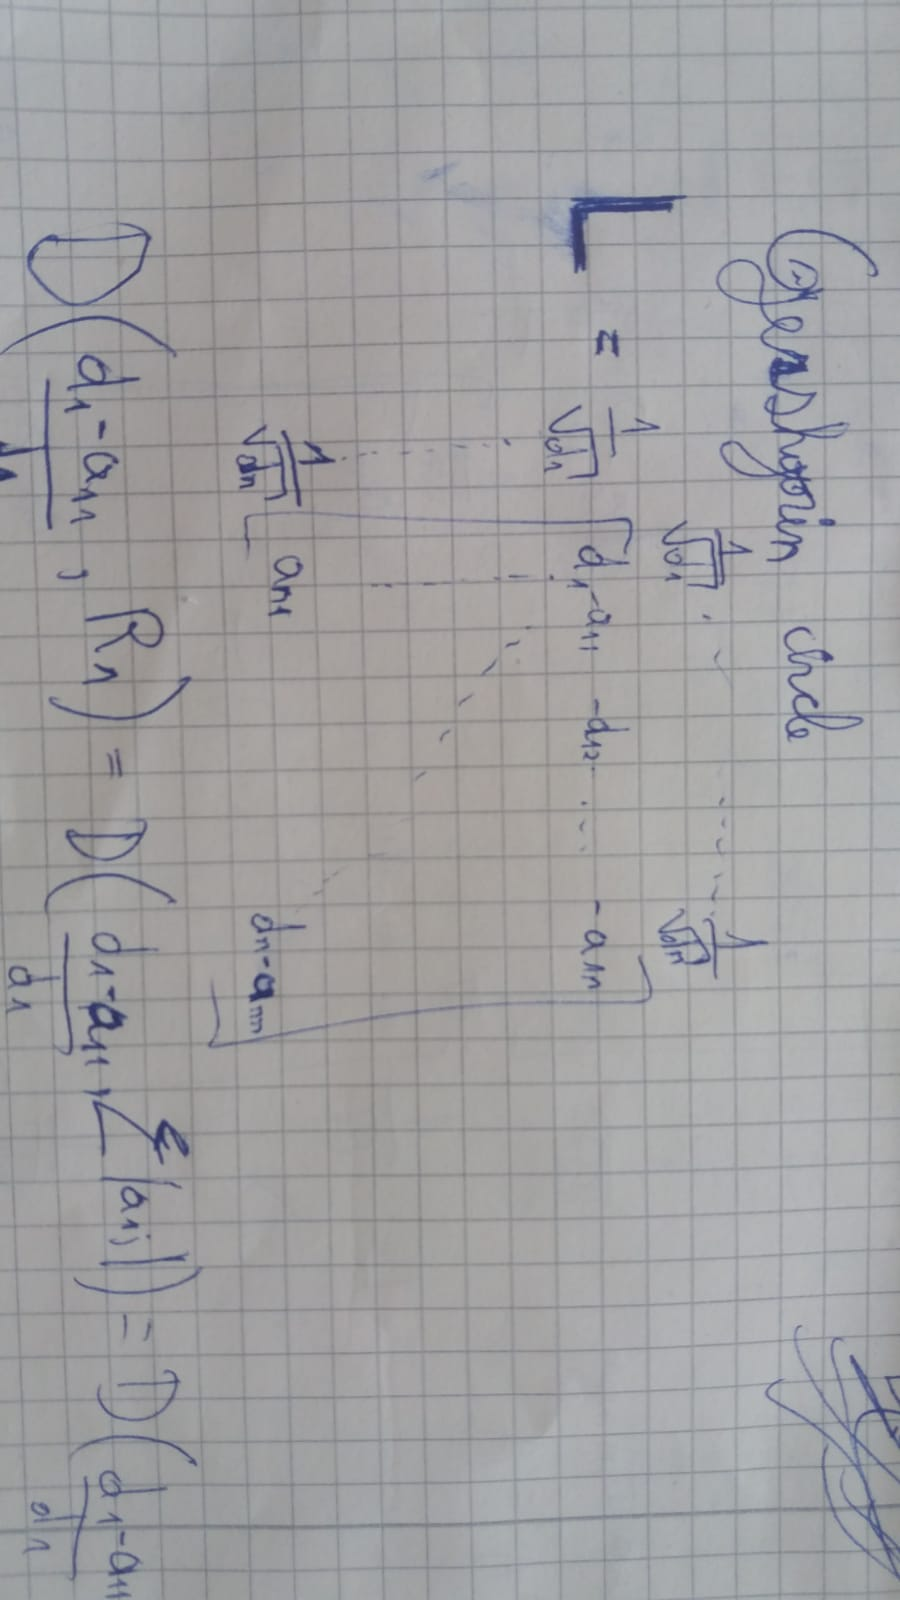
\includegraphics[scale=0.35, angle=90]{a10-ex1-a3.jpeg}
\end{figure}
\begin{figure}[h]
  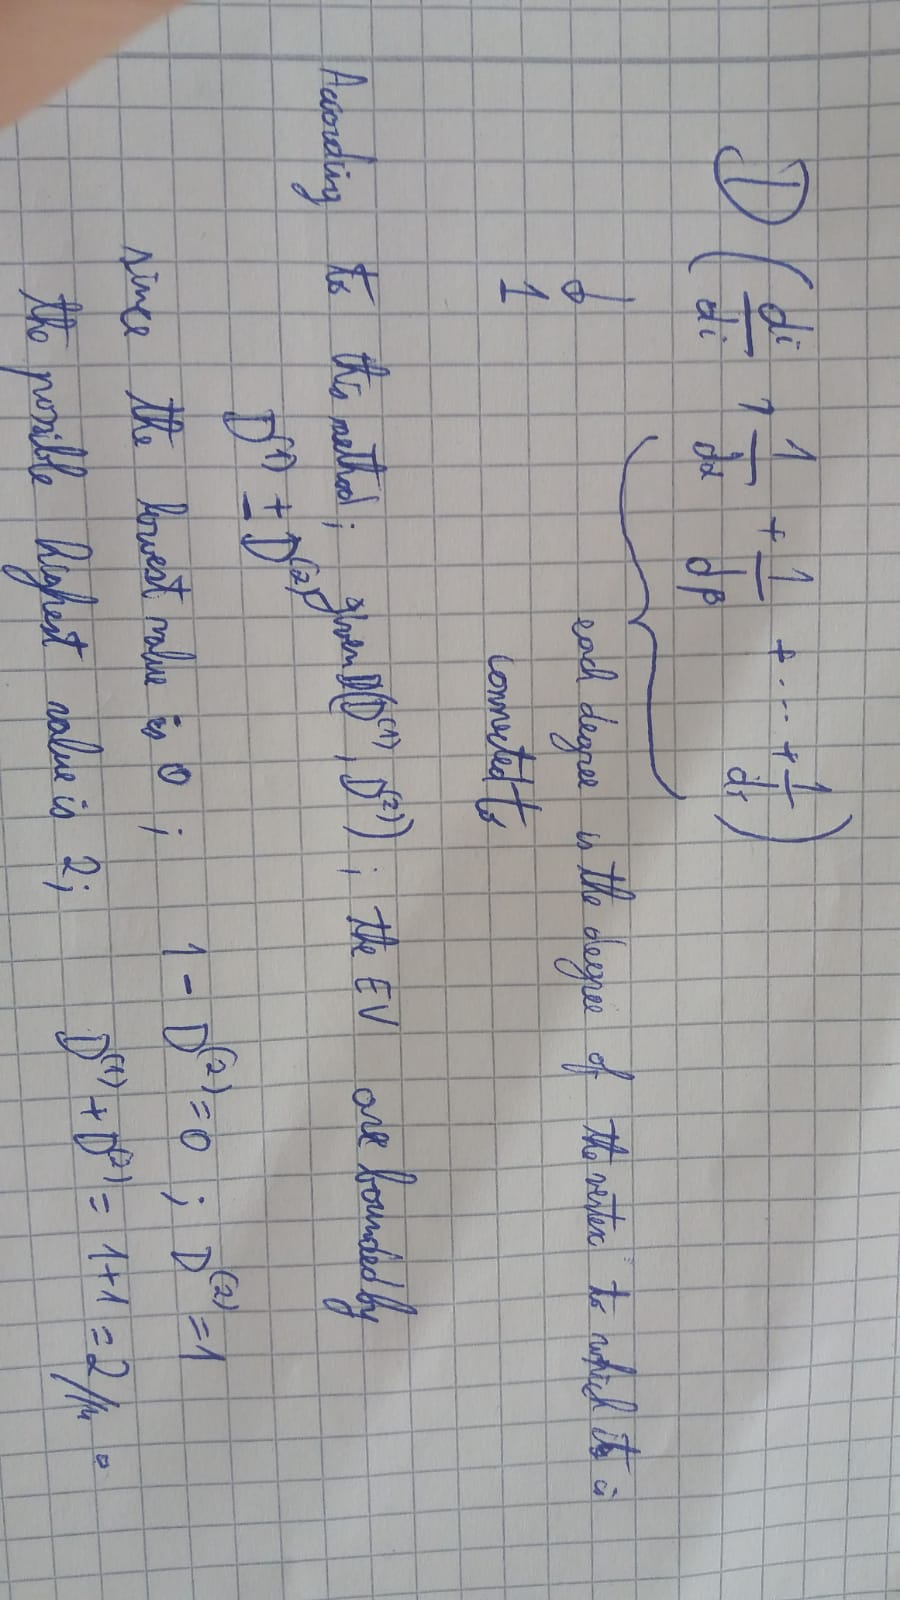
\includegraphics[scale=0.35, angle=90]{a10-ex1-a4.jpeg}
\end{figure}

% b
\item[(b)]
\begin{figure}[h]
  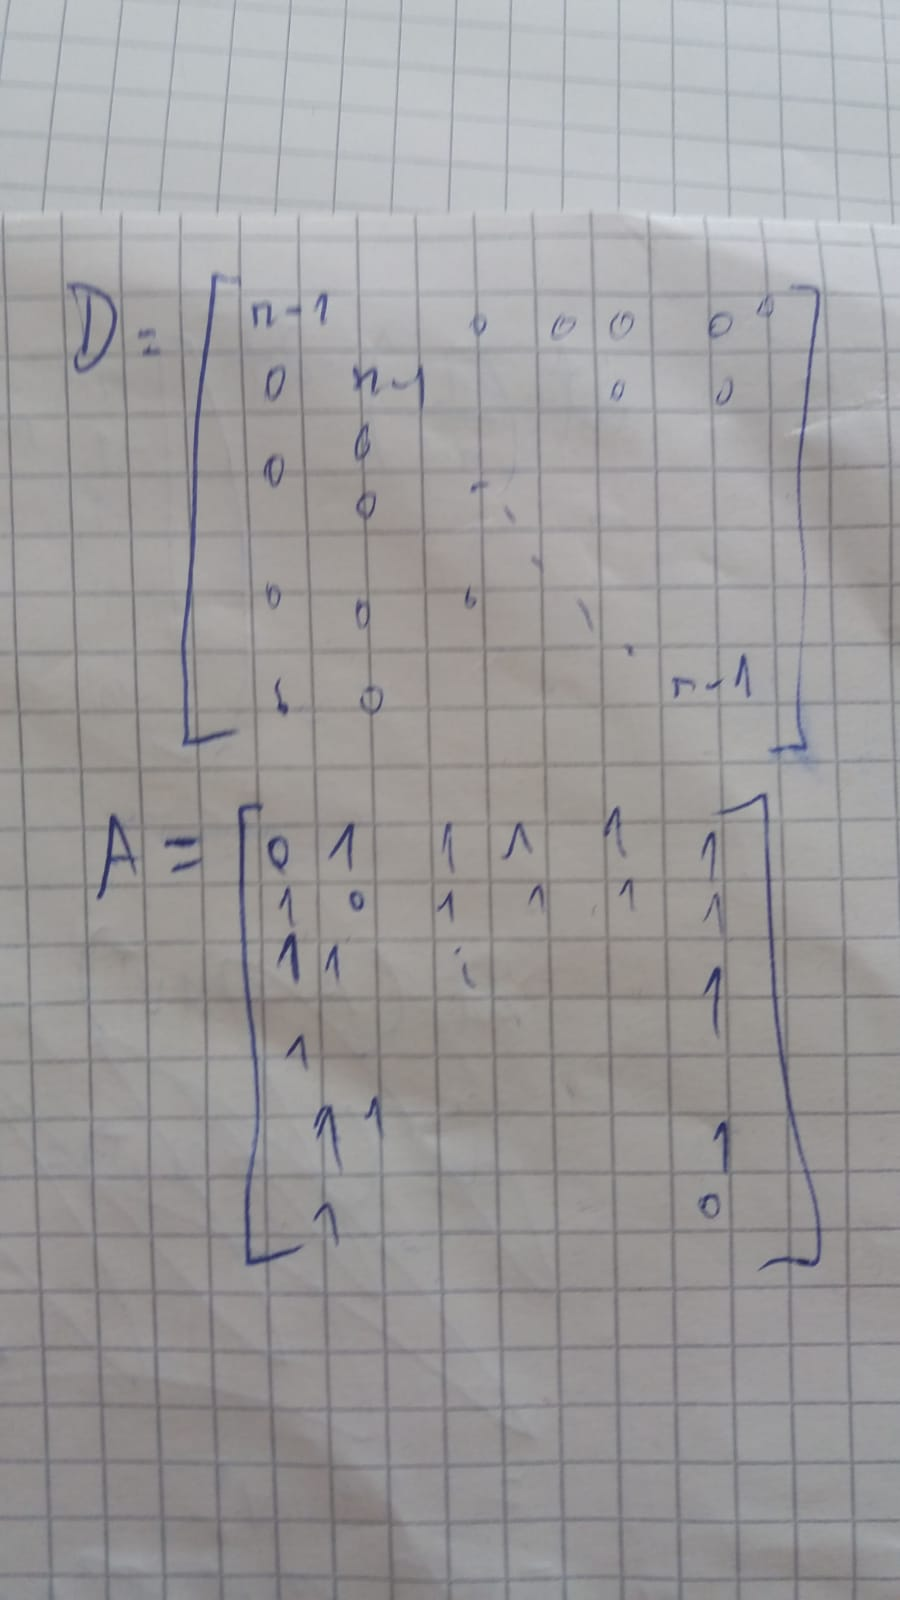
\includegraphics[scale=0.2]{a10-ex1-b1.jpeg}
\end{figure}
\begin{figure}[h]
  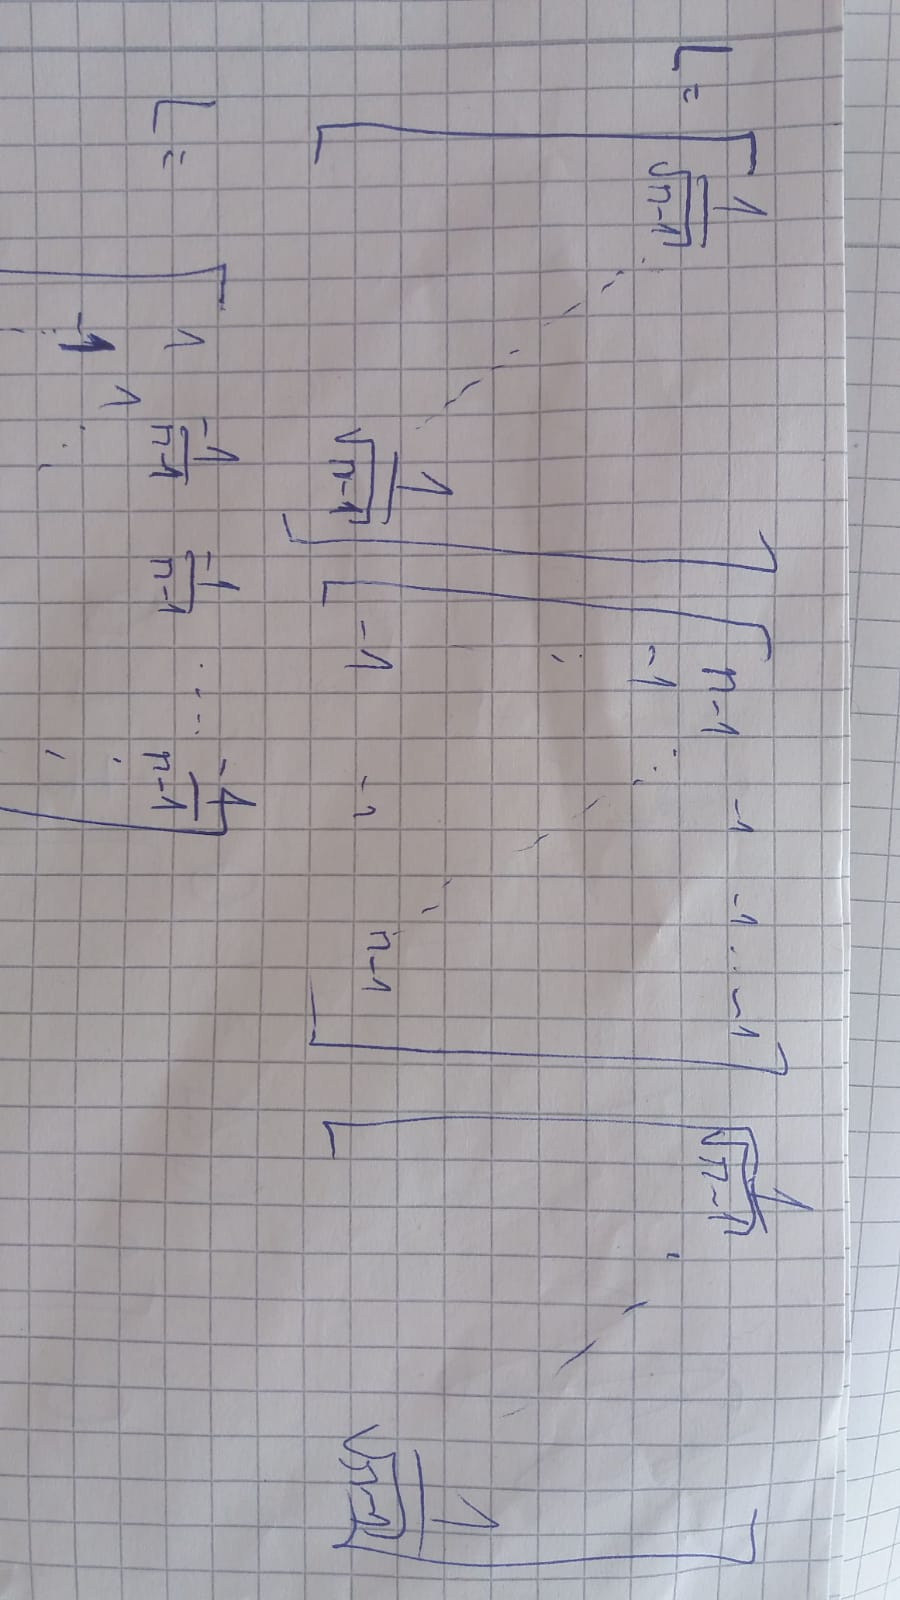
\includegraphics[scale=0.35, angle=90]{a10-ex1-b2.jpeg}
\end{figure}
\begin{figure}[h]
  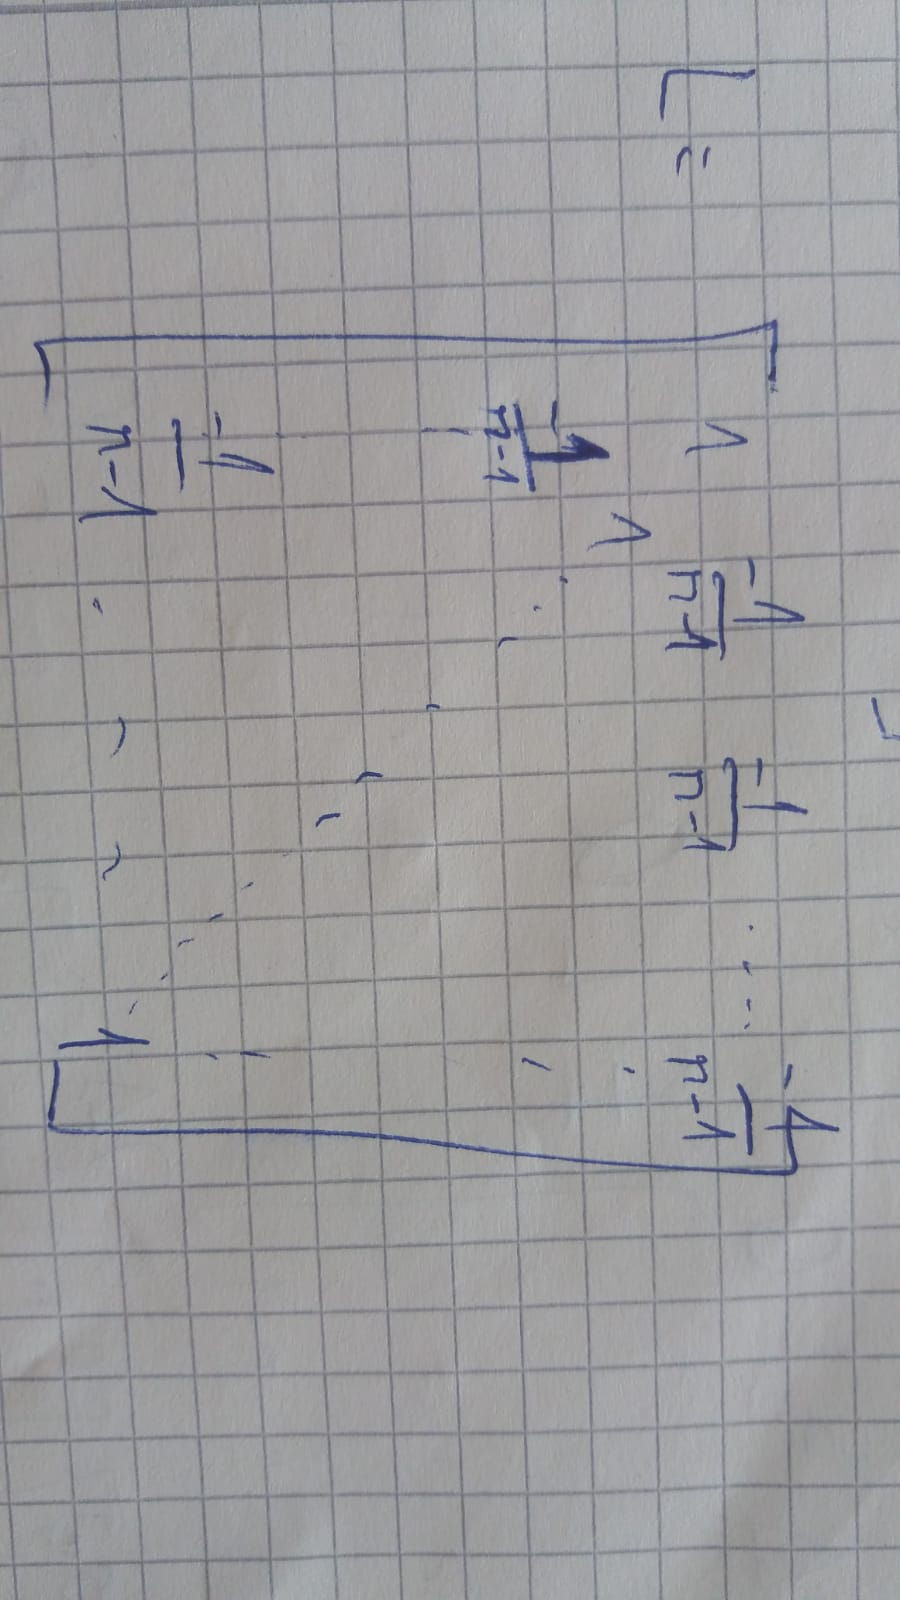
\includegraphics[scale=0.35, angle=90]{a10-ex1-b3.jpeg}
\end{figure}
\begin{figure}[h]
  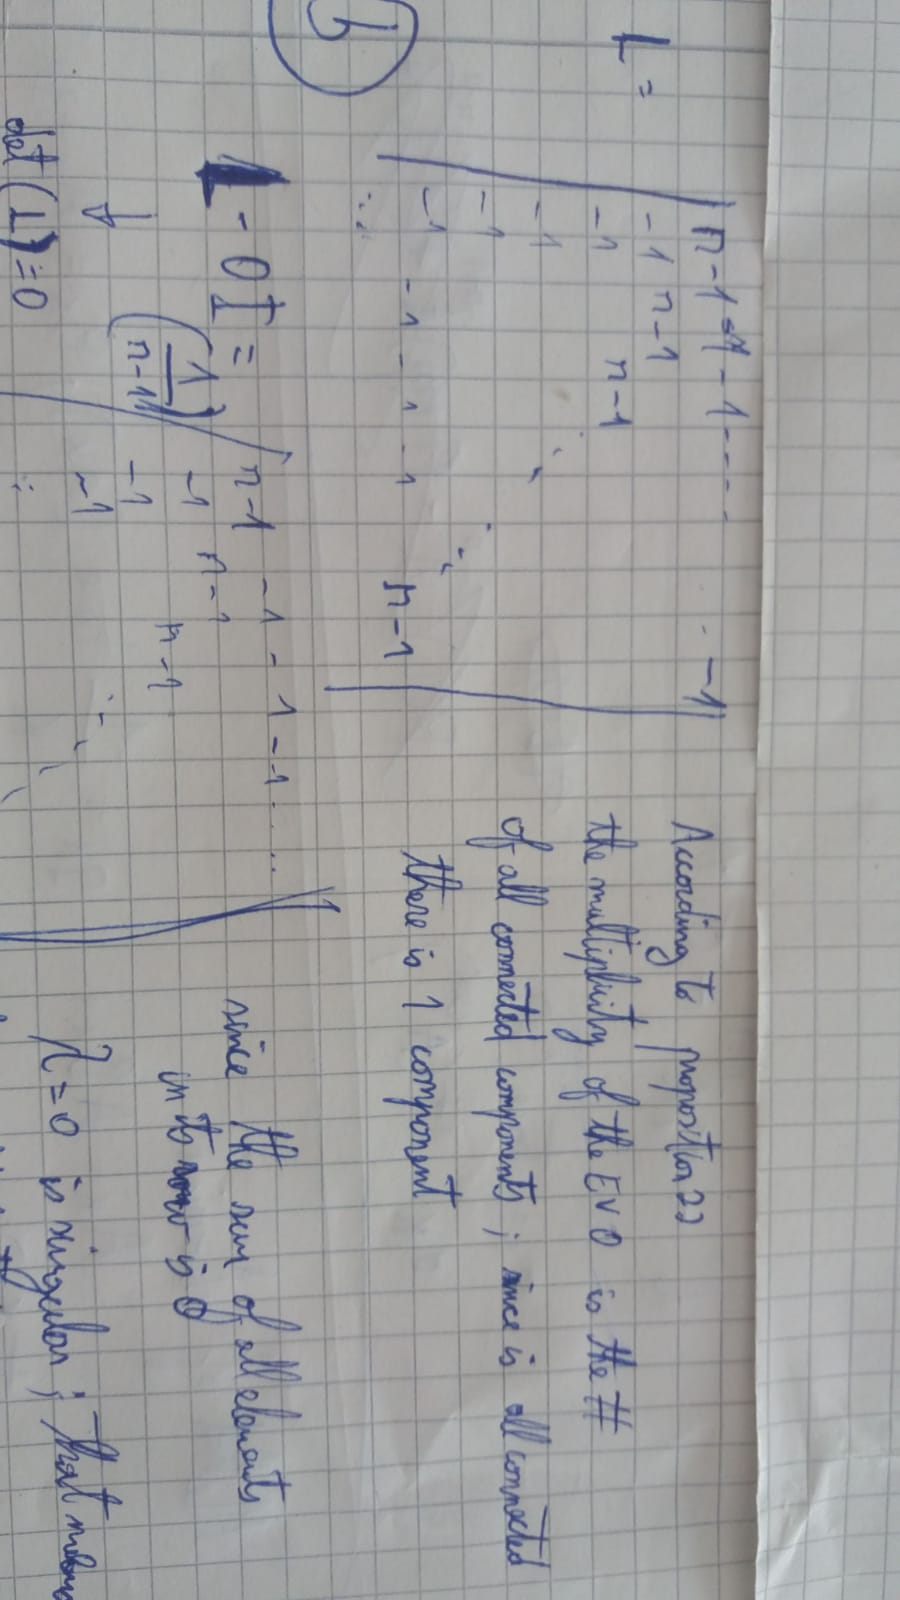
\includegraphics[scale=0.35, angle=90]{a10-ex1-b4.jpeg}
\end{figure}
\begin{figure}[h]
  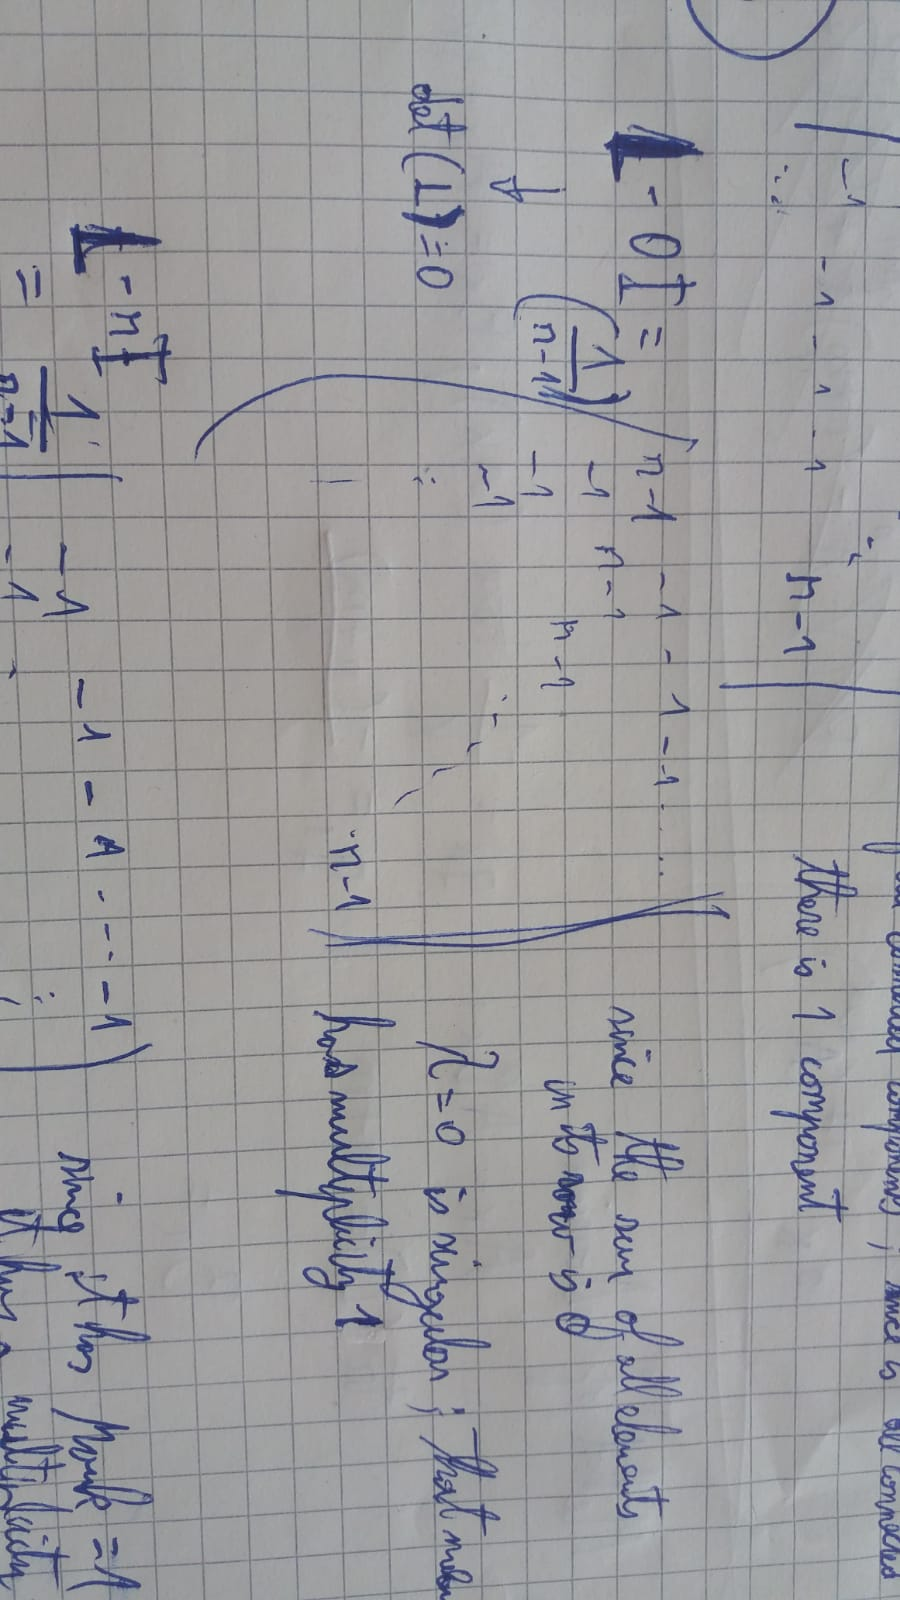
\includegraphics[scale=0.35, angle=90]{a10-ex1-b5.jpeg}
\end{figure}
\begin{figure}[h]
  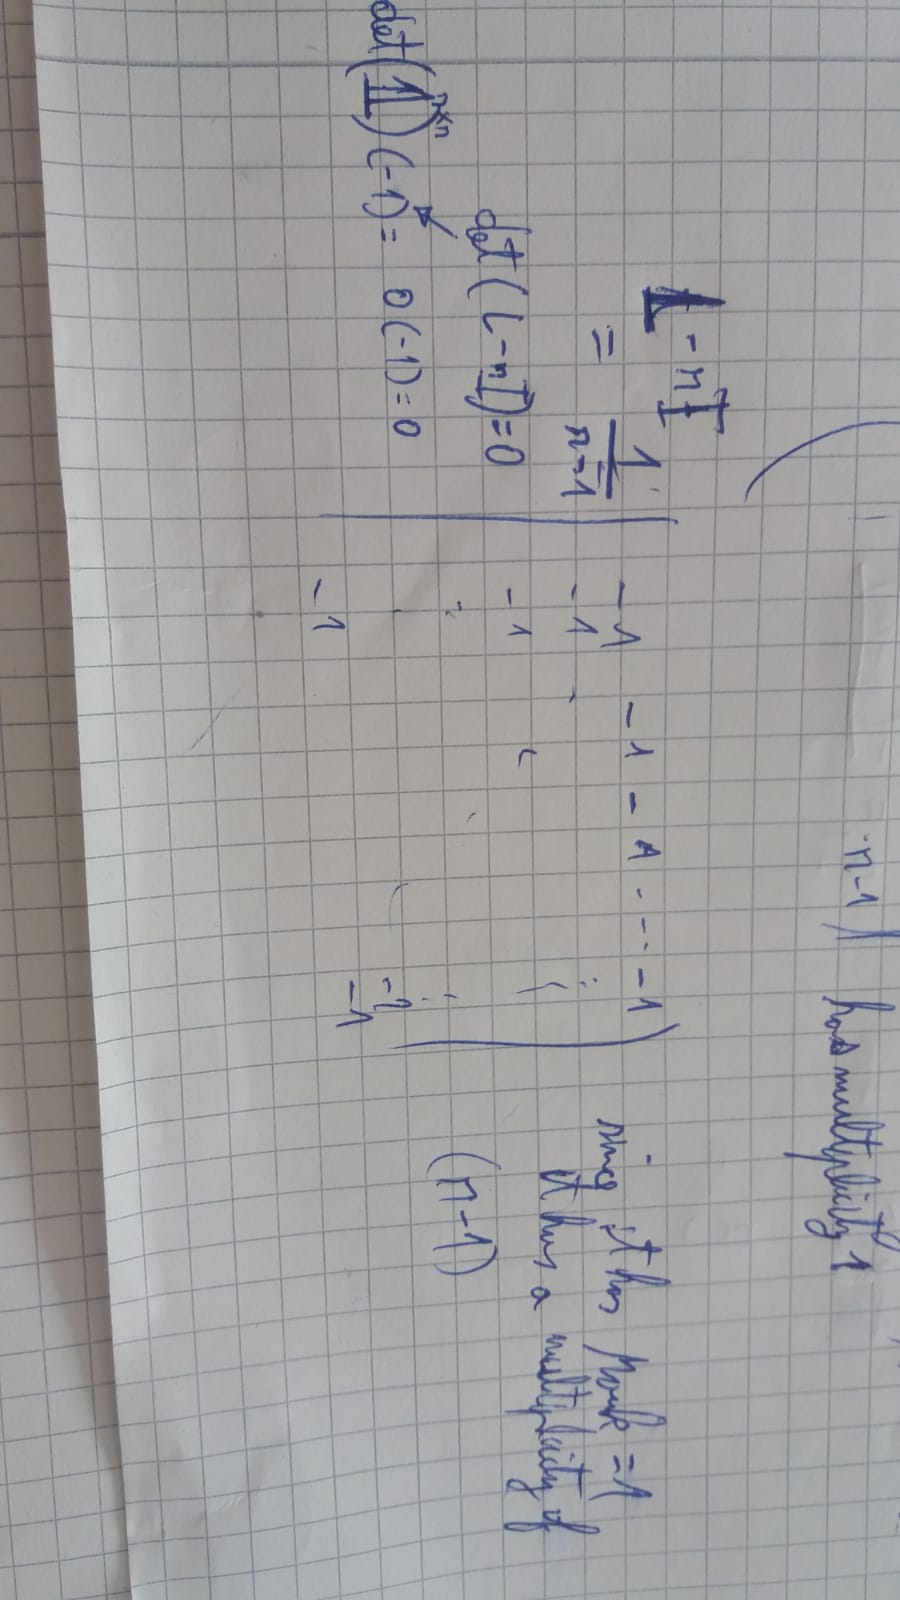
\includegraphics[scale=0.35, angle=90]{a10-ex1-b6.jpeg}
\end{figure}

% c
\item[(c)]
\begin{figure}[h]
  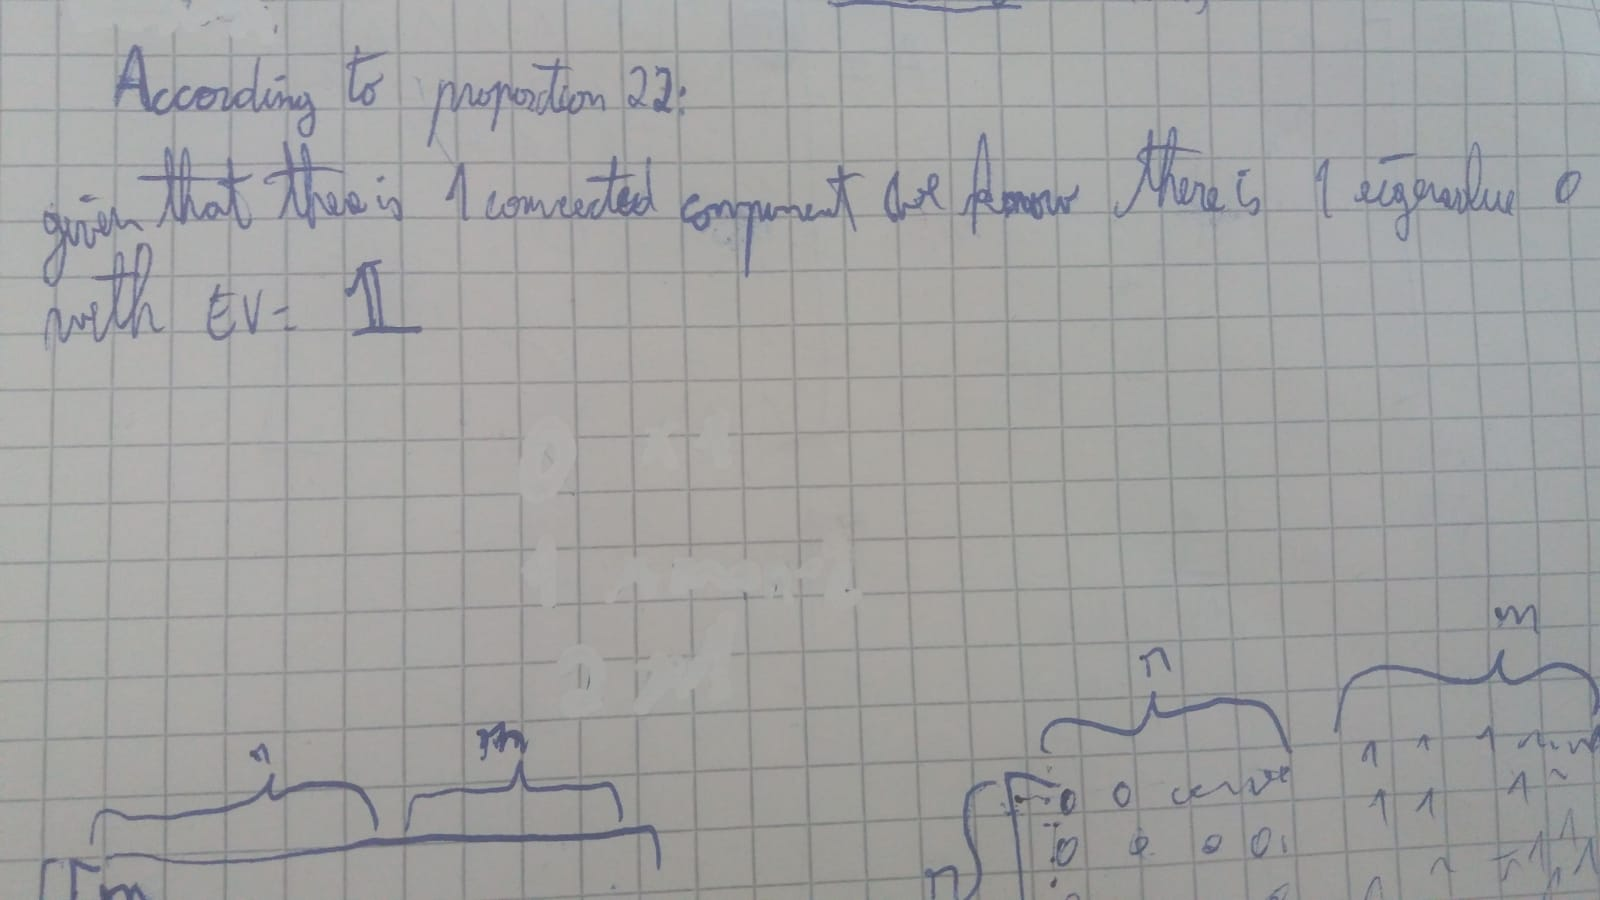
\includegraphics[scale=0.3]{a10-ex1-c1.jpeg}
\end{figure}
\begin{figure}[h]
  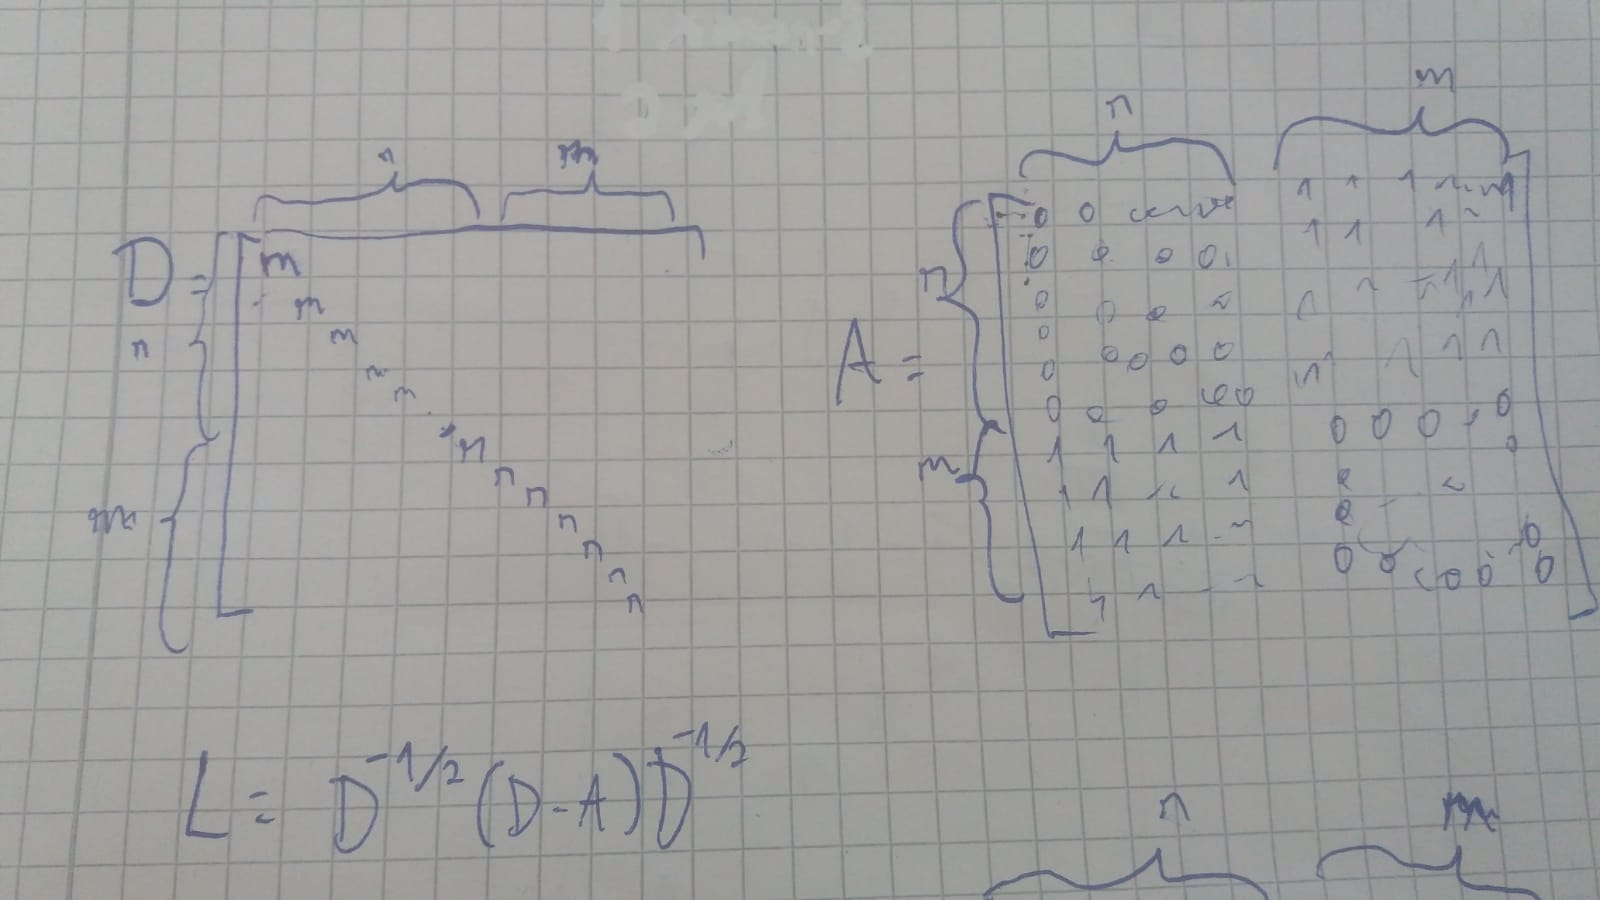
\includegraphics[scale=0.3]{a10-ex1-c2.jpeg}
\end{figure}
\begin{figure}[h]
  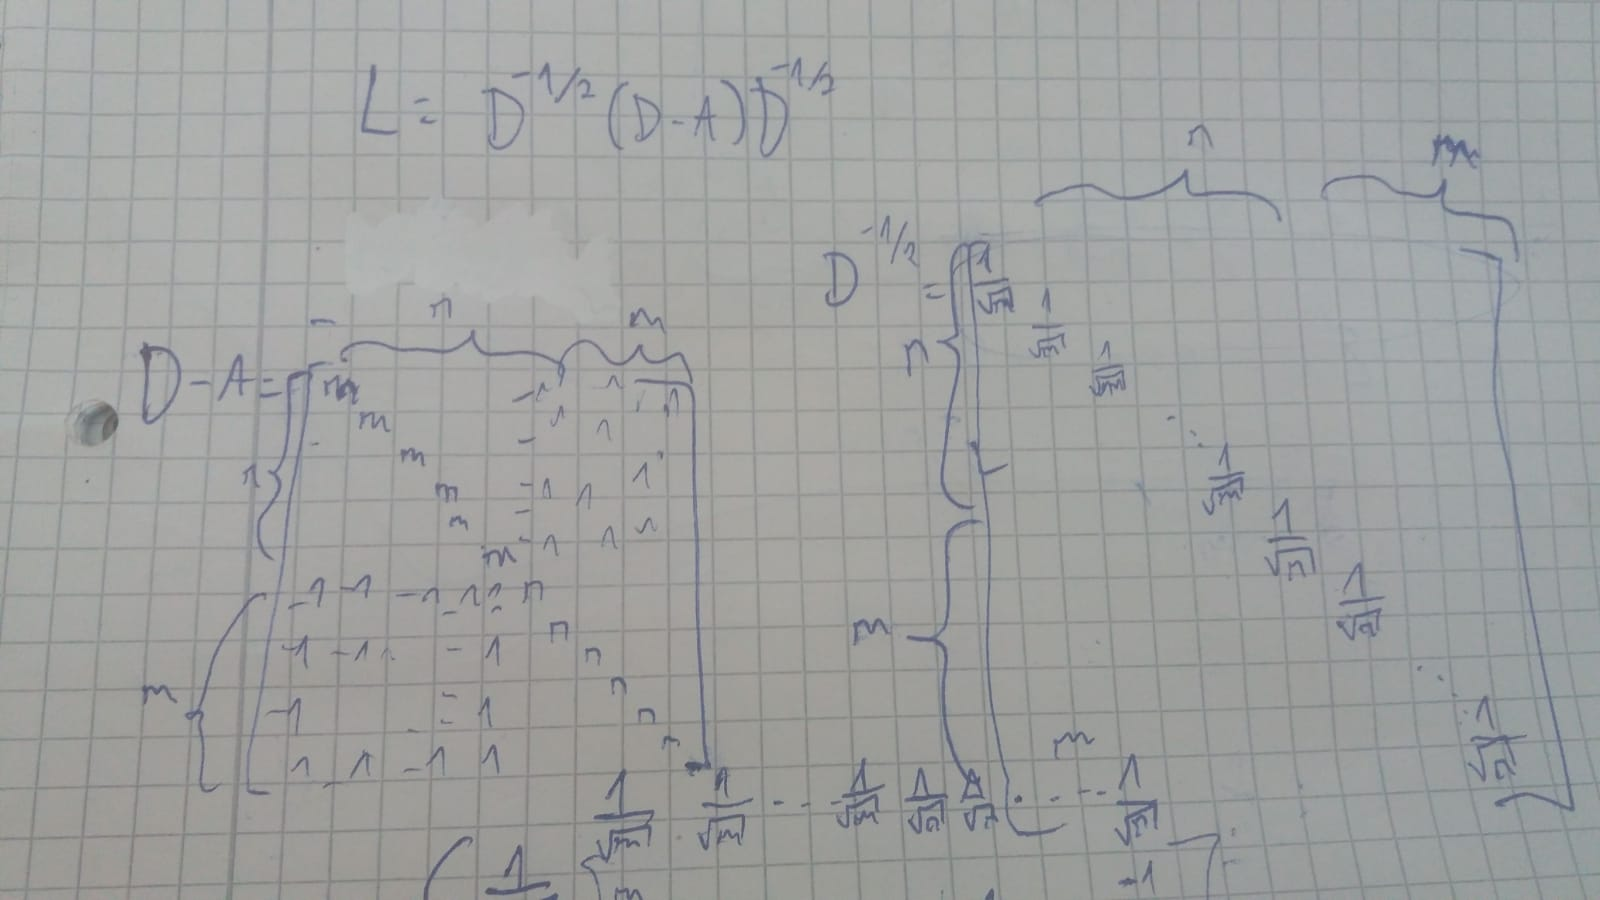
\includegraphics[scale=0.3]{a10-ex1-c3.jpeg}
\end{figure}
\begin{figure}[h]
  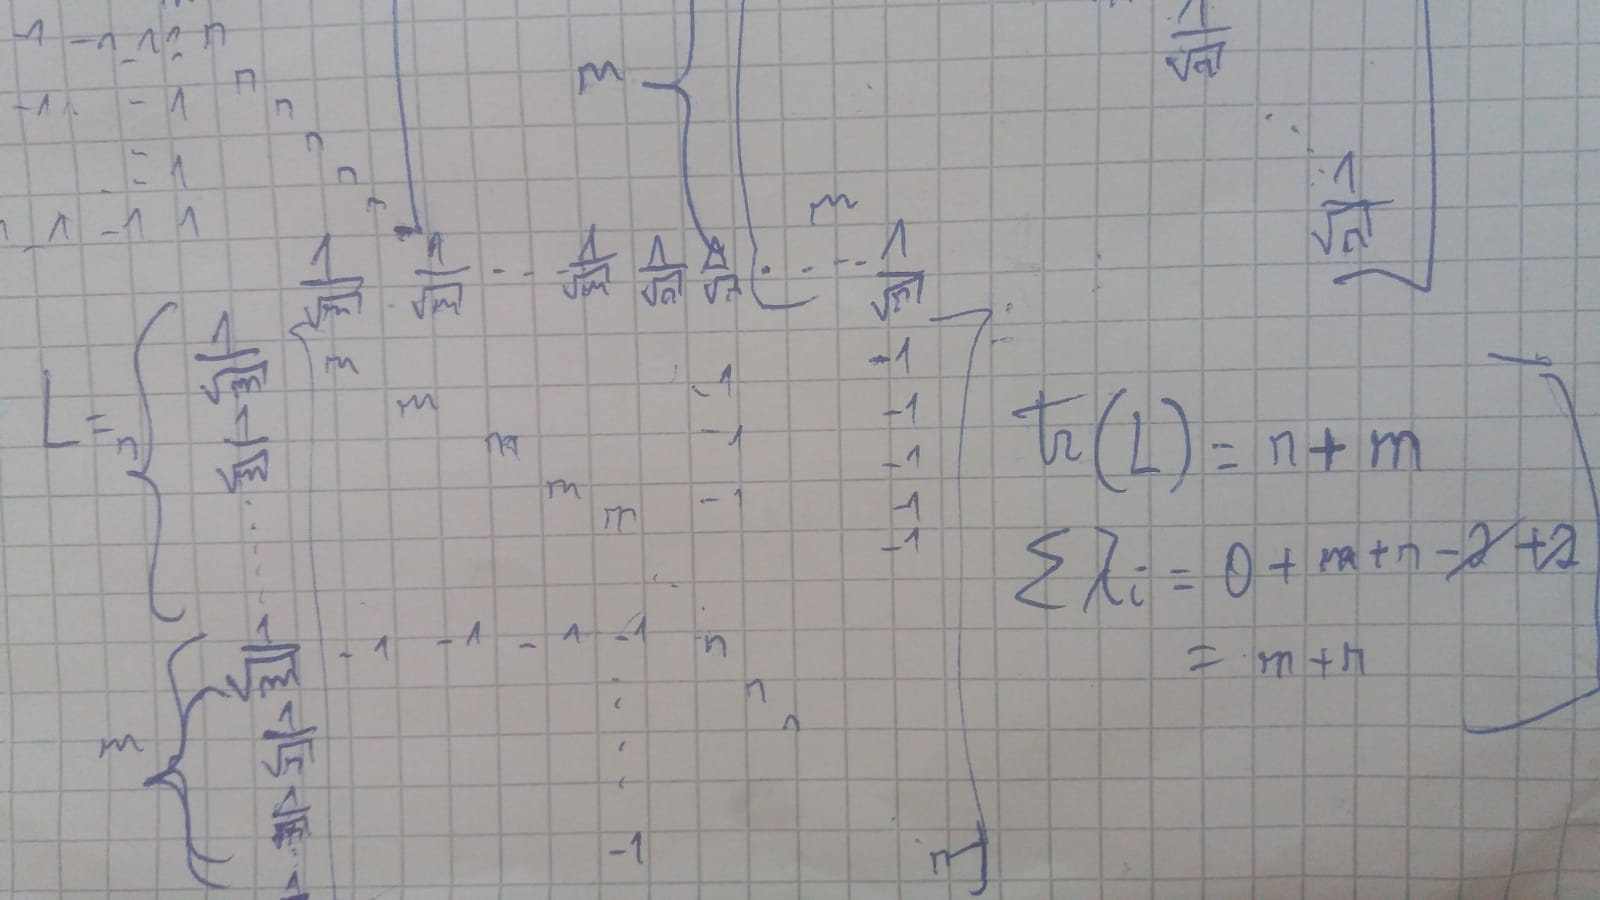
\includegraphics[scale=0.3]{a10-ex1-c4.jpeg}
\end{figure}

% d
\item[(d)]
\begin{figure}[h]
  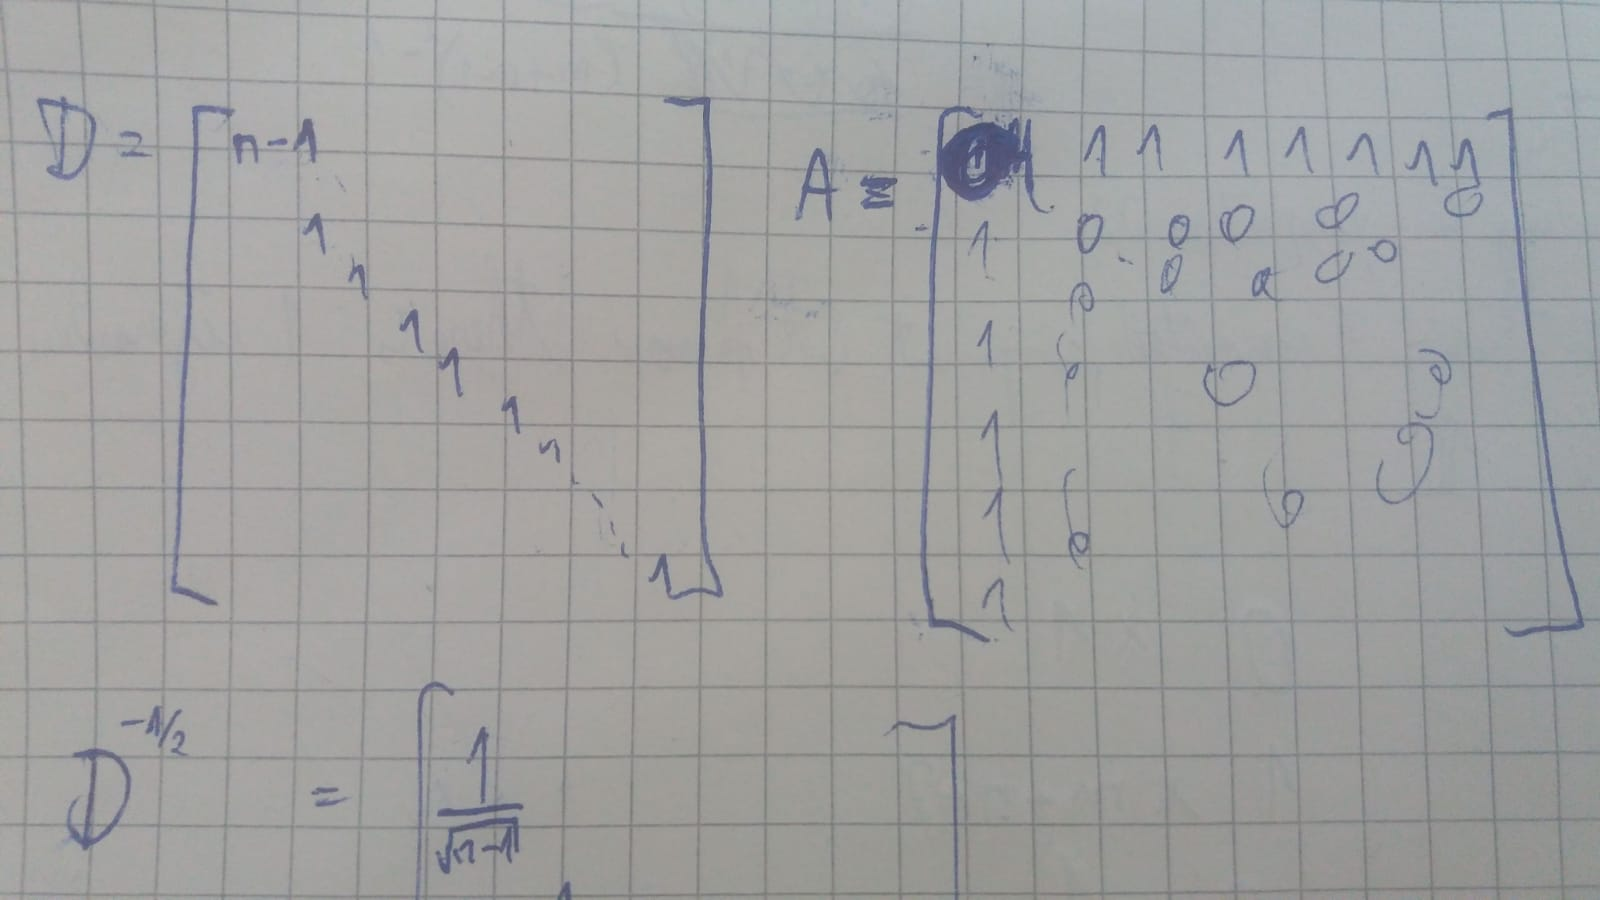
\includegraphics[scale=0.3]{a10-ex1-d1.jpeg}
\end{figure}
\begin{figure}[h]
  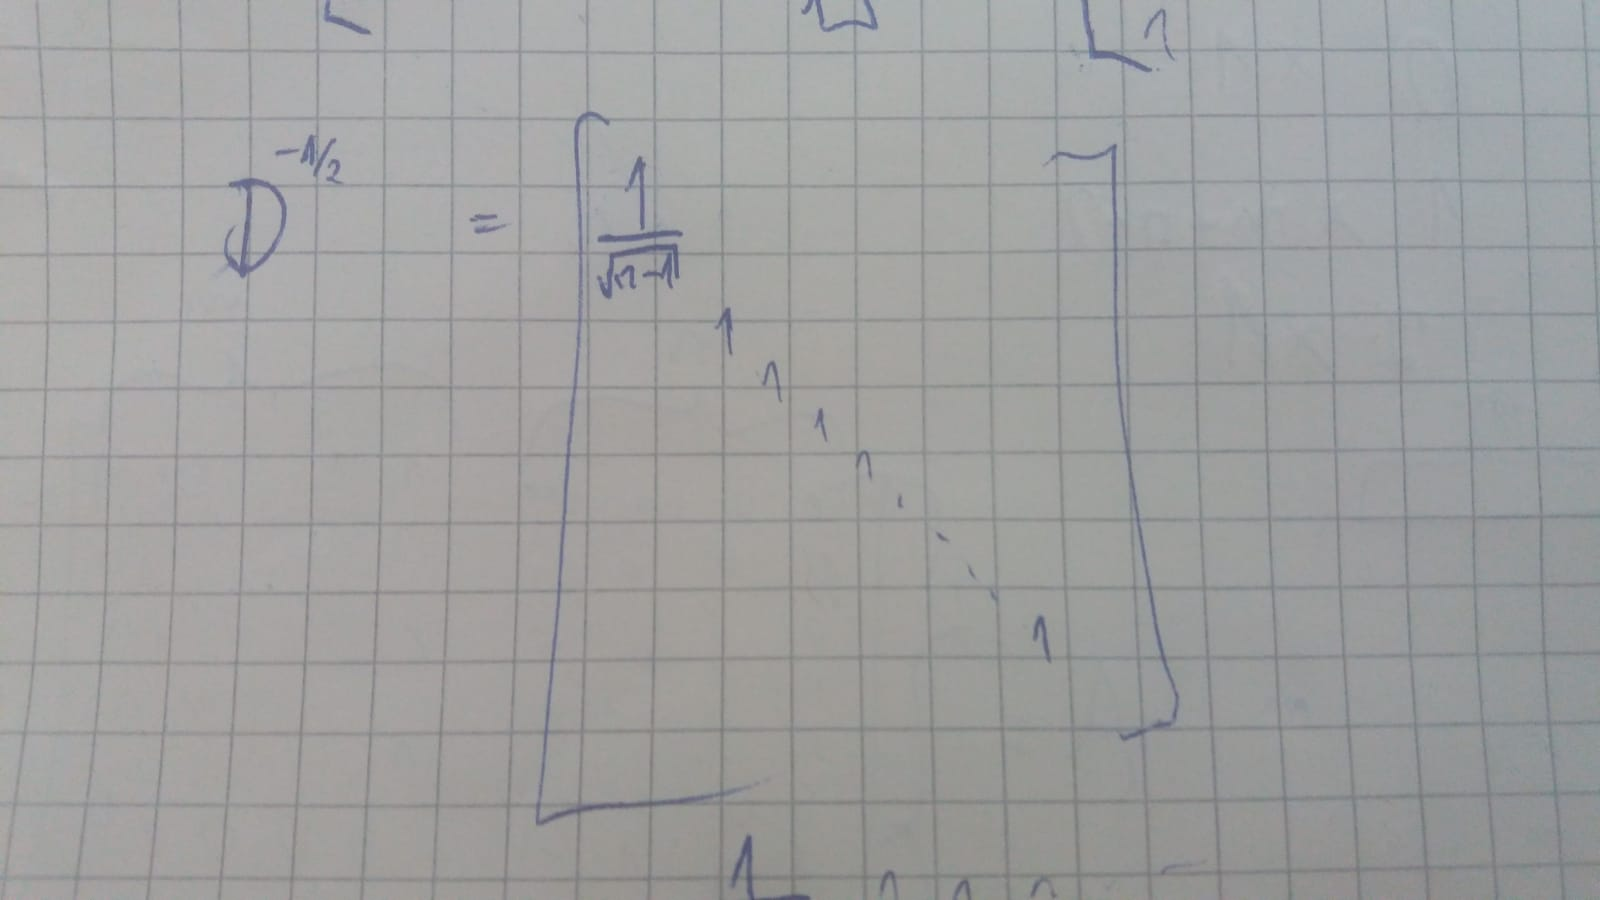
\includegraphics[scale=0.3]{a10-ex1-d2.jpeg}
\end{figure}
\begin{figure}[h]
  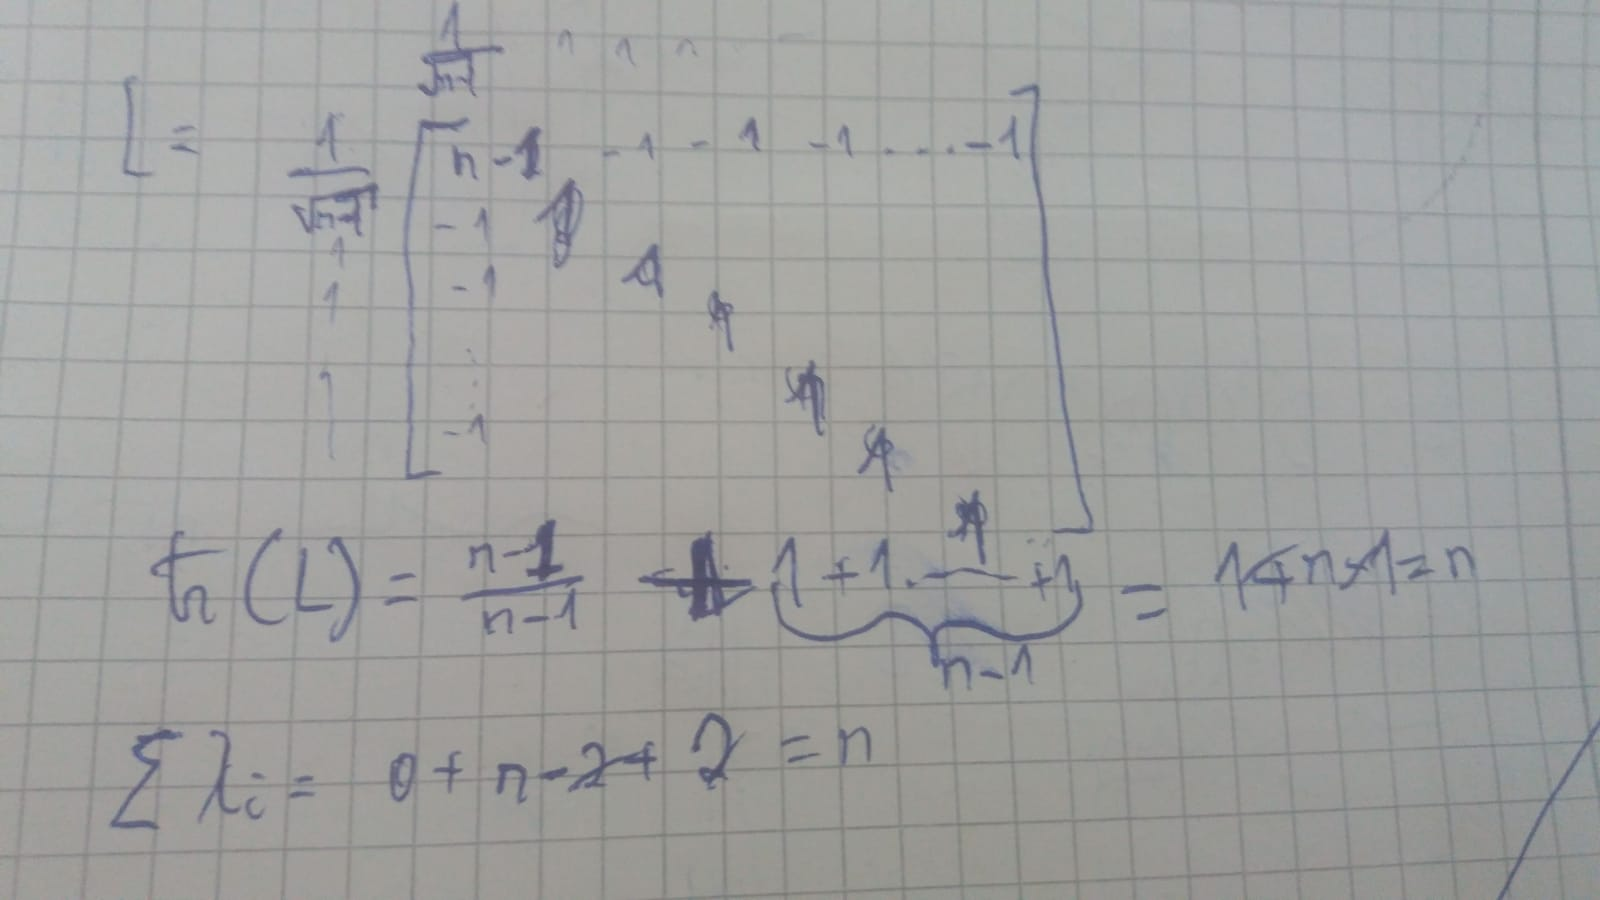
\includegraphics[scale=0.3]{a10-ex1-d3.jpeg}
\end{figure}

\end{description}

\end{document}
